\begin{comment}
\end{comment}

\chapter{Étude des codes polaires convolutifs}

Le problème de communication classique est défini comme suit.
Deux acteurs, 
qui se nomment Arthur et Béatrice pour faire changement\footnote{
  Une recherche en ligne vous démontrera que beaucoup d'attention a été donnée 
  à Alice et Bob. 
},
veulent échanger de l'information.
Dans ce cas,
supposons qu'Arthur cherchent à envoyer un message à Béatrice qui se trouve
des kilomètres plus loin.
Pour ce faire,
Arthur utilise son téléphone cellulaire et envoie un texto à Béatrice.
Une fois le message composé,
celui-ci est converti en une séquence de nombres binaires (des 0 et des 1)
qui sera transmise via des ondes radios jusqu'au téléphone de Béatrice
qui devra reconvertir la séquence de 0 et de 1 en message intelligible.

Cependant, 
l'histoire ne s'arrête pas là puisque lors de la transmission du signal
dans l'atmosphère, il est fort probable que celui-ci soit corrompu en 
raison d'une interaction indésirée.
En autre, 
cela peut être causé par la présence d'autres ondes ou d'un obstacle 
sur le trajet du signal.
La solution à ce problème est alors de transmettre une séquence de nombres binaires
plus longue que ce qui est nécessaire en espérant que l'information supplémentaire
nous aide à retrouver le message initial en cas d'erreur.

Dans ce chapitre,
je vais d'abord reformuler ce problème dans un langage mathématique plus formel.  
Par la suite, 
je vais présenter les réseaux de tenseurs,
un outil mathématique qui va m'être très utile pour décrire les codes polaires 
ainsi qu'une généralisation de ces derniers, les codes polaires convolutifs.
Ces codes sont très importants puisque les codes polaires sont au coeur 
de la technologie de communication 5G~\cite{bioglio_design_2021} et que toutes améliorations de ceux-ci
a un grand potentiel d'application.
À cet effet, le chapitre se termine par une présentation d'un article scientifique
dans lequel j'identifie les régimes où les performances des codes polaires convolutifs sont 
les plus impressionnantes.

\section{Communication classique et correction d'erreurs}

L'unité fondamentale de l'information est le bit.
Un bit prend la valeur 0 ou 1 et correspond à la quantité 
d'information acquiérie après avoir appris la réponse 
à une question ayant deux choix de réponses (oui et non par exemple).
Formellement, un bit est un élément du corps fini de cardinalité 2 noté $\bit = \qty{0, 1}$.
La multiplication dans $\bit$ est définie comme à l'habitude
et l'addition est définie modulo 2, soit que $1 + 1 = 0$.

Je m'intéresse au cas où Arthur veut transmettre une séquence 
de $k$ bits $\vb{x} \in \bit^k$ en utilisant un canal bruité $\canal$.
Dans cette thèse,
je vais me limiter à une définiton simple d'un canal bruité,
bien qu'il soit possible de généraliser cette notion. 
Le canal bruité que je considère est le canal binaire symétrique.
Celui-ci est une fonction probabiliste $\mathcal \canal_p: \bit \to \bit$
qui, après avoir reçu le bit $b$ comme entrée, 
retourne le même bit $b$ avec probabilité $1 - p$ et retourne le
bit opposé $1 + b$ avec probabilité $p$.
Il est commun de nommer $p$ la probabilité de renversement 
ou la probabilité d'erreur.

Dans le cas où $k > 1$ bits sont transmis via un canal bruité $\canal_p$,
un canal effectif $\canal_p^k$ composé de $k$ copies de $\canal_p$
est considéré.
Par exemple,
si le message $00000$ est transmis,
le message $01010$ est reçu avec probabilité $p^2(1 - p)^3$ 
tandis que le message $11111$ est reçu avec probabilité $p^5$.
De façon générale, 
la probabilité que le message original soit reçu sans erreur est de $(1 - p)^k$.
Cette probabilité décroit exponentiellement avec la taille du message 
et il est rapidement improbable que cela se produise.

Pour contrer ce problème,
chaque message original $\vb x \in \bit^k$ est encodé dans une autre séquence 
unique de bits $\vb{y} \in \bit^n$ telle que $n > k$.
Comme le nombre de messages dans $\bit^k$ est inférieur au nombre
de séquences dans $\bit^n$,
seul un sous-espace $\code \subset \bit^n$ est utilisé.
Ce sous-espace $C$ définit un code correcteur d'erreurs
de $k$ bits logiques et de $n$ bits physiques 
et un élément de $C$ est nommé mot-code.

\begin{table}[t]
  \caption{Exemple d'encodage de 2 bits vers 6 bits}
  \label{tab:exemple_encodage}
  \begin{center}
    \begin{tabular}[c]{cc}
      \textbf{Message} & \textbf{Mot-code} \\
      \hline
      00 & 000000 \\
      01 & 101010 \\
      10 & 010101 \\
      11 & 111111
    \end{tabular}
  \end{center}
\end{table}

Le tableau~\ref{tab:exemple_encodage} illustre un exemple de code correcteur
encodant 2 bits logiques à l'aide de 6 bits physiques.
En utilisant ce code correcteur,
Béatrice est en mesure de retrouver le message initial qu'Arthur lui a
envoyé s'il y a au plus une erreur qui affecte les 6 bits transmis. 
Par exemple, si le message 01 est transmis à l'aide du mot-code 
101010 et que la séquence 111010 est reçu, 
il est aisé, en comparant cette séquence avec les différents 
mots-codes, d'identifier le message envoyé. 
Par contre, 
si deux erreurs affectait le mot-code générant la séquence 111110, 
Béatrice concluerait à tord que le message 11 a été envoyé par Arthur.
L'opération qui consiste à essayer de retrouver le message original à partir
de la séquence reçue se nomme décodage 
et une erreur logique est une erreur à la suite du décodage.

Pour cet exemple,
la probabilité de transmettre un message de 2 bits sans encodage avec succès 
est de $(1 - p)^2$. 
En comparaison,
lorsque l'encodage de 6 bits est utilisé, 
la probabilité que Béatrice soit en mesure de retrouver le message original 
sans erreur logique est de $(1 - p)^6 + 6p(1 - p)^5$.
Ainsi, si $p \lesssim 0.22$, il est avantageux d'utiliser le code correcteur.

Le défi de la correction d'erreur est de construire des codes correcteurs 
qui réduisent considérablement la probabilité d'une erreur logique sans utiliser 
un trop grand nombre de bits supplémentaires.
À cet effet, c'est en 1948 que Claude Shannon a démontré la plus grande valeur 
de rendement $R = k/n$ qui peut être transmise 
via un canal bruité~\cite{shannon_mathematical_1948}.
Plus précisement,
la capacité $\capacite$ d'un canal bruité est le rendement maximum 
que peuvent transmettre plusieurs copies du canal tel que la probabilité d'une 
erreur logique tend vers 0 lorsque $n \to \infty$.
Autrement dit,
pour un canal de capacité $\capacite$, 
il existe une famille de codes $\qty{C_i}_{i\in\mathbb N}$ avec 
$k_i / n_i \to \capacite$ telle que la probabilité d'une erreur de 
décodage décroit exponentiellement avec $i$.

La capacité d'un canal est calculé à partir de l'information mutuelle~\footnote{
  Les concepts importants de la théorie de l'information, dont l'entropie
  et l'information mutuelle sont présentés à l'annexe~\ref{chap:theo_info}.
} 
selon
\begin{equation}
  \capacite = \max_{\Pr_X(x)} I(X ; Y),
\end{equation}
avec $X$ la variable aléatoire transmise et $Y$ la variable aléatoire reçue.
Dans ce cas,
l'information mutuelle $I(X ; Y)$ est interprété comme la fraction maximale
de bits non erronés qui peuvent être reçus par bit envoyé.
Cette quantité dépend généralement de la probabilité d'envoyer chaque bit
et il est alors optimal de choisir la probabilité qui maximise l'information mutuelle.
Lors de l'introduction aux codes polaires à la fin de ce chapitre,
j'utiliserai l'information mutuelle pour comparer la performance de divers canaux.

Pour le canal binaire symétrique $\canal_p$, 
il est prouvé~\cite{shannon_mathematical_1948} que l'information mutuelle
est maximisée par une probabilité uniforme sur $X$. 
La capacité est alors
\begin{equation}
  \capacite(\canal_p) = 1 - H_2(p)
\end{equation}
avec l'entropie binaire $H_2(p) = -p \log(p) - (1 - p)\log(1 - p)$~\footnote{
  Pour alléger le texte, je n'inclus pas les preuves qui se retrouvent facilement 
  dans la littérature.
}. 
La figure~\ref{fig:capacite_canal} illustre que la capacité du canal binaire symétrique 
est nulle à $p = 0.5$.
En effet, un canal ayant une probabilité d'erreur de $0.5$ retourne 
chacune des séquences de bits avec la même probabilité 
et cela, peu importe le message transmis.
Un tel canal est donc inutilisable.
En contrepartie, la capacité est maximale à $p = 0$ et $p = 1$.
Lorsque la probabilité d'erreur est nulle,
il n'y a aucun avantage à utiliser un code correcteur 
et il suffit de transmettre le message directement.
Par contre, il est un peu plus surprenant que la capacité soit maximale lorsque la probabilité
d'erreur est de 1.
Cependant, en utilisant un tel canal, 
il suffit de renverser chacun des bits reçus pour retrouver le message transmis sans erreur.
De même, 
un canal avec une probabilité d'erreur $1 - p$ est équivalent à un canal de probabilité d'erreur $p$
après avoir renversés tous les bits reçus.
C'est pourquoi, 
les études numériques de cette thèse se concentre sur des plages de probabilités entre 0 et 0.5.

\begin{figure}
  \begin{center}
    \includegraphics{figures/capacite_canal.pdf}
  \end{center}
  \caption{Capacité du canal binaire symétrique selon la probabilité d'erreur}
  \label{fig:capacite_canal}
\end{figure}

Il est important de noté que l'article de Shannon n'inclut aucune construction de codes 
correcteurs permettant d'atteindre la capacité du canal binaire symétrique.
En effet, les codes polaires sont les premiers codes correcteurs découverts 
pour lesquels il existe un algorithme de décodage efficace permettant d'atteindre 
la capacité d'un canal~\cite{arikan_channel_2009}. 
En ce sens, il s'agit d'une famille de codes qui optimise le compromis en réduction du bruit 
et rendement.

Avant d'introduire les codes polaires et les codes polaires convolutifs,
je vais faire un petit détour à la prochaine section pour introduire les réseaux de tenseurs.
Cet outil mathématique me permettera alors d'exprimer de façon plus concise la construction
de ces codes et les algorithmes de décodage correspondant.

\section{Réseaux de tenseurs}
\label{sec:reseaux_tenseurs}

Les réseaux de tenseurs sont une représentation graphique de problèmes d'algèbre linéaire
particulièrement utile pour des systèmes de grandes tailles.
Dans cette thèse, 
je vais me limiter à introduire les notions essentielles à la construction des 
codes polaires et des codes polaires convolutifs.
Pour cela, 
je vais me concentrer sur les réseaux de tenseurs comme un outil d'algèbre linéaire 
et je ne discuterai pas des considérations plus physiques (corrélations, entropie, etc) 
qui accompagnent généralement une introduction du sujet.
Pour plus de détails,
il existe plusieurs articles d'introduction~\cite{bridgeman_hand-waving_2017, baker_methodes_2021} aux réseaux de tenseurs qui couvrent de nombreuses applications de cet outil principalement en physique du solide,
mais également pour des domaines comme l'informatique quantique et l'apprentissage automatique. 

Intuitivement, 
un tenseur est la généralisation d'une matrice.
En effet,
tout comme une matrice, 
un tenseur peut être compris comme une boite de nombres identifiés par une liste d'indices. 
Pour les matrices,
il suffit d'une paire d'indices pour identifier un élément,
alors qu'un nombre arbitraire d'indices peut être utilisé pour un tenseur. 
Le rang d'un tenseur est le nombre d'indices utilisé pour identifier un élément.
Par exemple, 
un scalaire $s$ est un tenseur de rang 0, 
un vecteur $v_i$ est un tenseur de rang 1 
et une matrice $m_{ij}$ est un tenseur de rang 2.

Une des opérations parmi les plus importantes sur les tenseurs est la contraction.
La contraction de deux tenseurs est la généralisation du produit matricielle.
Avant de définir la contraction,
il est intéressant de revenir un peu sur le produit matricielle.

Pour une matrice $A$ de dimension $l \times m$ et une matrice $B$ de dimension $m \times n$,
les éléments du produit matricielle $C = AB$ sont donnés par
\begin{equation}
  C_{ij} = \sum_{k=0}^{m - 1} A_{ik} B_{kj}.
\end{equation}
Chacun des éléments de $C$ est obtenu en faisant 
la somme sur le second indice de $A$ et le premier de $B$ 
en fixant la valeur des indices restant.
Le dernier indice de $A$ et le premier indice de $B$ forment 
alors un indice commun de la paire $(A, B)$.
La contraction de deux tenseurs de rangs arbitraires est définie 
de la même façon.
Par exemple, 
le tenseur $C$, dont les éléments sont
\begin{equation}
  C_{hijkl} = \sum_{r} A_{hrij} B_{klr},
\end{equation}
est la contraction du tenseur $A$ de rang 4
et du tenseur $B$ de rang 3, 
ayant comme indice commun
le deuxième indice de $A$ et le troisième de $B$\footnote{
En pratique, pour calculer la contraction de deux tenseurs, 
une série d'opérations de remodelage et de permutation des indices 
est effectuée pour représenter les tenseurs comme des matrices et 
ainsi profiter des nombreuses optimisations développées pour les algorithmes
de multiplication matricielle.
Je considère cependant qu'il s'agit d'un détail d'implémentation 
et je ne m'attenderai pas sur ce point.}.
Une contraction n'est pas limitée à un seul indice.
En effet,
pour les mêmes tenseurs $A$ et $B$ le tenseur $D$ ayant les éléments
\begin{equation}
  D_{hik} = \sum_{r} \sum_{s} A_{hris} B_{ksr}
  \label{eq:contraction_somme}
\end{equation}
est une contraction de deux indices de $A$ et $B$.

\begin{figure}[t]
  \begin{center}
    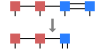
\includegraphics{figures/contraction_reseau}
  \end{center}
  \caption{
    La contraction de deux tenseurs d'un réseau.
    Cette contraction des tenseurs bleus à la droite du réseau
    en un nouveau tenseur de rang 3 correspond à l'équation~\eqref{eq:contraction_somme}.
  }
  \label{fig:contraction_reseau}
\end{figure}

Dans les sections~\ref{sec:codes_polaires} et~\ref{sec:codes_polaires_conv},
j'utiliserai plusieurs dizaines voir centaines de tenseurs pour 
représenter des distributions de probabilité.
Dans ce cas, 
la notation de sommation devient inutilisable 
en raison du nombre trop important de tenseurs et d'indices.
Pour contourner ce problème,
j'utiliserai une notation graphique pour les tenseurs.
C'est cette représentation graphique qui porte le nom de réseaux de tenseurs.

Un réseau de tenseur est défini par un graphe $G = (\tenseurs, \aretes)$\footnote{Je fais 
un rappel des notions de théorie des graphes à l'annexe~\ref{chap:theo_graphe}.} où $\tenseurs$ 
est un ensemble de tenseurs et $\aretes \subseteq (\tenseurs \times \tenseurs) \cup \tilde{\tenseurs}$ 
est un ensemble d'arêtes fermées, $\tenseurs \times \tenseurs$, reliant deux tenseurs 
et d'arêtes ouvertes, $\tilde \tenseurs = \qty{\qty{T} : T \in \tenseurs}$, comprenant un seul tenseur.
Une arête $a \in \aretes$ est connectée à un tenseur $T \in \tenseurs$ si $T \in a$.
Le rang d'un tenseur $T \in \tenseurs$ correspond au degré de $T$ dans $G$,
soit le nombre d'arêtes connectées à $T$.
Ainsi, chaque arête connectée à $T$ correspond à un indice de $T$.

Une arête fermée correspond à un indice commun entre deux tenseurs à contracter.
Suite à la contraction d'un indice commun, le réseau est modifié comme 
illustré à la figure~\ref{fig:contraction_reseau}.
Lors de la contraction d'une paire de tenseurs dans un réseau,
le nombre d'arêtes ouvertes du réseau est conservé.
La contraction d'un réseau de tenseurs est ainsi une séquence de contractions 
de paires de tenseurs jusqu'à ce qu'il ne reste qu'un seul tenseur avec des arêtes ouvertes.
Pour ce faire, 
il est important de considéré l'ordre des contractions pour minimiser la taille 
des tenseurs intermédiaires puisque cela peut avoir un impact considérable sur la mémoire
requise et le temps de calcul.
En effet,
il est possible que ces deux quantités augmentent exponentiellement avec le nombre 
de tenseurs et d'arêtes dans le réseau initial.
Trouver l'ordre de contraction optimal est un problème appartenent 
à la classe de complexité $\sharp P$\footnote{Je fais un rappel des notions de la 
théorie de la complexité à l'annexe~\ref{chap:complexite_calcul}. Dans ce cas, 
il est suffisant de comprendre qu'il s'agit d'un problème très difficile même 
en utilisant une grande quantité de ressources numériques.}~\cite{biamonte_tensor_2015}. 
Heureusement,
pour les codes polaires et les codes polaires convolutifs,
un ordre de contraction efficace se présente naturellement.


\section{Codes polaires}
\label{sec:codes_polaires}


C'est en 2009 que Arikan introduit les codes polaires~\cite{arikan_channel_2009}.
Le concept fondamentale derrière la construction des codes polaires est la polarisation
des canaux bruités.
Cette technique permet de convertir deux canaux bruités similaires en un canal moins bruité
et un canal plus bruité.
Ainsi,
un ensemble de canaux presque sans bruit et un ensemble presque inutilisable
sont obtenues en répétant itérativement cette approche à partir de plusieurs canaux similaires.
Ce qui est remarquable est que la fraction de canaux de faible bruit créés ainsi
tend vers la capacité des canaux initiaux.
En combinant cela au fait qu'il existe un algorithme efficace de décodage des codes polaires,
nous obtenons une famille de codes aux performances très prometteuse.
Dans le reste de cette section,
je vais d'abord décrire plus en détail la procéssus de polarisation des canaux avant
d'introduire la construction des codes polaires.
Finalement, je vais présenter un décodeur pour ces codes.
Je ferai tout cela en utilisant le formaliste des réseaux de tenseurs.

\begin{figure}[t]
  \begin{center}
    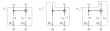
\includegraphics{figures/polarisation.pdf}
  \end{center}
  \caption{Polarisation d'une paire de canaux}
  \label{fig:polarisation}
\end{figure}

Je vais décrire un canal à partir de sa fonction de poids. 
Ainsi,
le canal binaire symétrique $\canal_p$ est représenté par la fonction de poids
\begin{equation}
  W(y|x) =
  \begin{cases}
    1 - p & \text{si } x = y,\\
    p & \text{si } x \neq y.\\
  \end{cases}
\end{equation}
Cette fonction représente la probabilité de recevoir $y$ si $x$ a été transmis.

Pour la construction des codes polaires,
des canaux plus généraux $W(\vb y | x)$,
où $\vb y \in \qty{0, 1}^m$ est un vecteur de $m$ bits,
sont considérés.
De plus, 
l'analyse se limite aux canaux composés de canaux binaires symétriques.
Dans ce cas, l'information mutuelle d'un canal décrit par $W(\vb y | x)$
est maximisée par une probabilité uniforme des valeurs de $x$.
La capacité est alors~\footnote{
  Sauf indication contraire, les logarithmes dans cette thèse sont calculés en base 2.
}
\begin{align}
  \capacite(W) 
  = I(X ; Y)
  &= \sum_{\vb y \in \qty{0, 1}^m}\sum_{x \in \qty{0, 1}} 
  \Pr(x, y) \log\qty(\frac{\Pr(x, y)}{\Pr(x) \Pr(y)})\notag\\
  &= \sum_{\vb y \in \qty{0, 1}^m}\sum_{x \in \qty{0, 1}} 
  \frac{1}{2}W(\vb y | x) \log\qty(\frac{2 W(\vb y | x)}{W(\vb y | 0) + W(\vb y | 1)})
  \label{eq:capacite_symetrique}
\end{align}
puisque $\Pr(x = 0) = \Pr(x = 1) = 1/2$.

La première étape de la polarisation est de combiner 
deux copies du canal binaire symétrique $W_1$ en un nouveau canal à 2 bits selon 
\begin{equation}
  W_2(\vb y_1^2 | \vb u_1^2) = W_1(y_2 | u_2) W_1(y_1 | u_1 + u_2),
\end{equation}
comme illustré à la figure~\ref{fig:polarisation}.
Dans cette section, je suis la littérature sur la correction d'erreurs
classique et j'utilise la notation $\vb x_i^j = (x_i, x_{i + 1}, \ldots x_j)$.
Le canal $W_2$ est obtenu en transformant l'entrée $(u_1, u_2)$ vers $(u_1 + u_2, u_2)$.
Cette transformation est l'analogue classique de la porte logique CNOT très utilisée 
en informatique quantique.

Le canal $W_2$ est ensuite décomposé en un mauvais canal $W_2^{(1)}$ et un bon canal $W_2^{(2)}$.
Pour ce faire,
les bits $u_1$ et $u_2$ sont transmis de façon successive.
D'abord, 
le bit $u_1$ est transmis en ignorant la valeur de $u_2$. 
Le mauvais canal,
\begin{equation}
  W_2^{(1)}(\vb y_1^2 | u_1) 
  = \sum_{u_2 \in \qty{0, 1}} W_2(\vb y_1^2 | u_1^2) 
  = \frac{1}{2}\sum_{u_2 \in \qty{0, 1}} W_1(y_2 | u_2) W_1(y_1 | u_1 + u_2),
\end{equation}
est obtenu en supposant qu'il est équiprobable que $u_2 = 0$ et $u_2 = 1$.

Pour retrouver la valeur de $u_1$ transmise par ce canal, 
la valeur de $u_2$ est estimée selon $W_1(y_2 | u_2)$. 
La probabilité de succès est de $1 - p$. 
Ensuite, 
la valeur de $u_1$ est estimée selon $W(y_1 | u_1 + u_2)$.
En supposant la bonne valeur de $u_2$, 
la probabilité de succès de cette étape est également de $1 - p$.
Ainsi, la probabilité totale de succès est de $(1 - p)^2 = 1 - 2p + p^2$,
ce qui est inférieure à la probabilité de succès $1 - p$ de $W$.

\begin{figure}
  \begin{center}
    \includegraphics{figures/capacite_polarisation.pdf}
  \end{center}
  \caption{Comparaison de la capacité des canaux polarisés.}
  \label{fig:capacite_polarisation}
\end{figure}

Le bon canal est construit en supposant que la valeur de $u_1$ est connue,
soit parce qu'elle est fixée initialement ou qu'elle a été retrouvée avec succès
après l'utilisation du mauvais canal.
La fonction de poids du bon canal est alors
\begin{equation}
  W_2^{(2)}(\vb y_1^2, u_1 | u_2) 
  = W_2(\vb y_1^2 | u_1^2) 
  = W_1(y_2 | u_2) W_1(y_1 | u_1 + u_2),
\end{equation}
où la valeur de $u_1$ est connue. 
Dans le cas où $u_1 = 0$, 
utiliser ce canal est équivalent à envoyer deux copies de $u_2$. 
Ainsi, 
s'il y a une seule erreur, alors $y_1 \neq y_2$ et il est possible de détecter l'erreur.
Une erreur doit donc affecter chacun des bits pour que celle-ci ne soit pas détecter.
Cela a une probabilité $p^2$ ce qui est bien inférieure à la probabilité d'erreur $p$ du
canal $W_1$.
Une logique similaire s'applique lorsque $u_1 = 1$.

La capacité des différents canaux est calculée à partir 
de l'équation~\eqref{eq:capacite_symetrique}
et est illustrée à la figure~\ref{fig:capacite_polarisation}.












\section{Codes polaires convolutifs}
\label{sec:codes_polaires_conv}

\section{Article : Comparaison de la profondeur et de la largeur des codes polaires convolutifs}

Cet article ayant pour titre original \textit{Depth versus Breadth in Convolutional Polar Codes}
a été publié en 2018 dans la cadre de la conférence \textit{IEEE Information Theory Workshop}.
Dans celui-ci,
nous comparons plusieurs généralisations des codes polaires basées sur la construction 
des codes polaires convolutifs CITATION DAVID ET ANDREW.
Ces généralisations varient la largeur des codes polaires en utilisant des portes 
de polarisation à plus de 2 qubits 
et varient la profondeur en ajoutant des couches convolutives 
de portes de polarisation à chaque niveau.
Ces deux modifications ne changent la complexité que par un facteur multiplicatif constant.

Le résultat principal de l'article est qu'augmenter la largeur des codes 
nuit aux performances alors qu'augmenter la profondeur augmente les performances.
Lorsque le nombre d'opérations nécessaires au décodage est pris en compte,
il est optimal de choisir une largeur et une profondeur de 2.



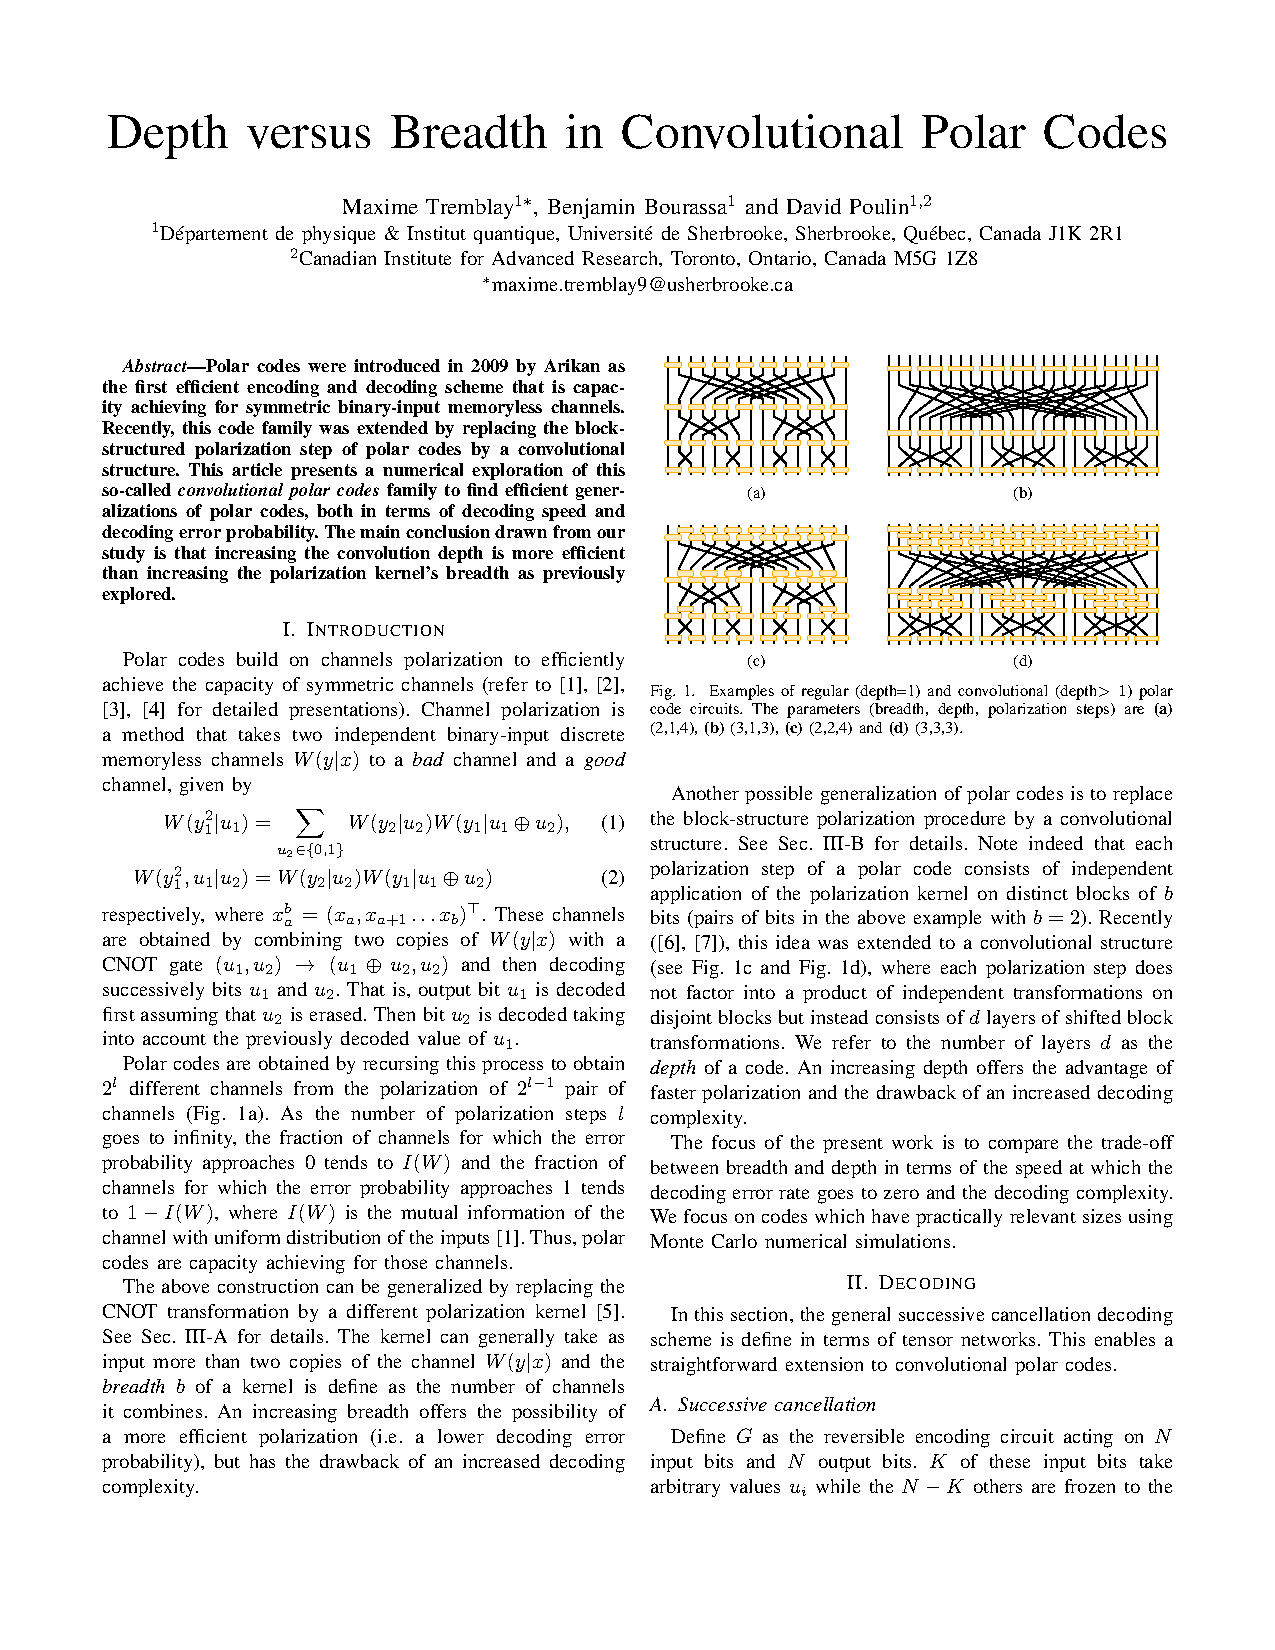
\includepdf[pages=-]{articles/conv_polar_codes.pdf}
